\begin{tcolorbox}[enhanced,breakable,colback=Black!5!lightgray,colframe=black!75!black,coltitle=white,title=Standard error of the mean]
It can be challenging to get an intuitive understanding of power, because the computations needed to calculate it are not straightforward. A key statistic is the standard error of the mean, also known as the SEM, usually shortened to standard error (SE). This can be thought of as an index of the variability of an estimate of the mean from a sample. If you imagine taking numerous samples from a population, and estimating the mean from each one, you will end up with a distribution of means; these estimates of the mean are much more variable for small than for large samples. The SE is the standard deviation of the estimates of the mean, and it is crucially dependent on the sample size.
This follows from the formula for the SE, which is computed as the SD divided by the square root of N.

The test statistic, \emph{z} in this instance, which is used to derive a p-value, uses the SE as a denominator, and so will also be influenced by sample size. The \emph{z} score is defined as:

z = (M - \(\mu\))/SE

The bigger the N, the smaller the SE, the more precise the measurement, and the higher the power of the statistical test. Note that the value entered into these equations is the \emph{square root} of N. It follows that improvement in precision from adding extra participants to a study is greatest at small sample sizes: as shown in the figure below, the SE is approximately halved in increasing the sample size from 10 to 40, whereas changes are much smaller in going from 110 to 140 participants.

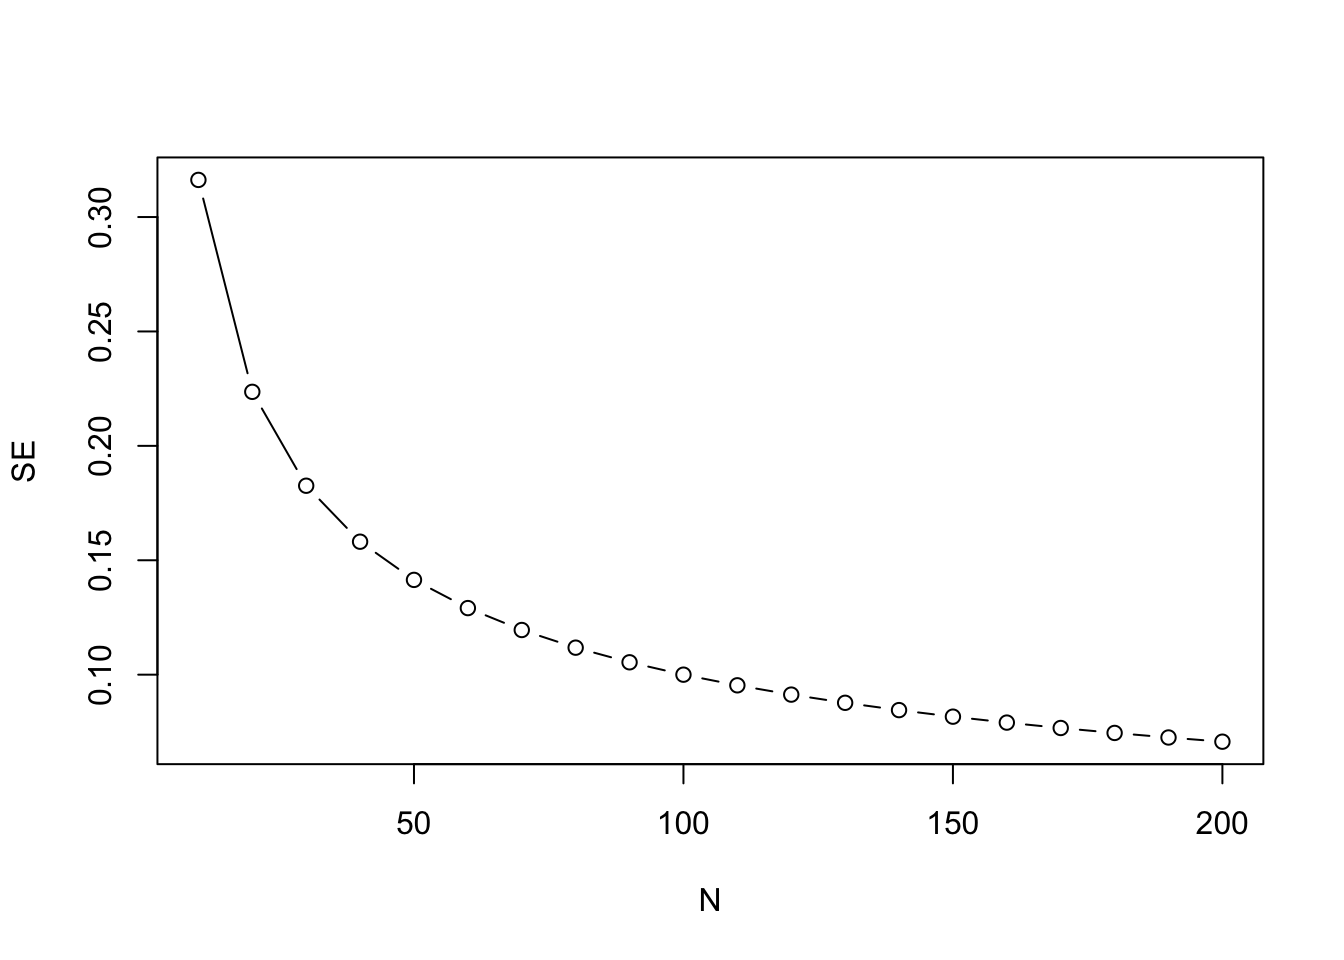
\includegraphics[width=0.6\linewidth]{images_bw/demoSE}\captionof{figure}{Plot showing how SE reduces with sample size (N) in a nonlinear fashion}\label{SEMbyN}
\end{tcolorbox}

